We already know the behaviour of a linked list, and if we are progrogramming a Singly linked list it means that we need just information about the next node and the value of the current node, so we need to use a struct called Node with a pointer to the next element, and a int value (the value of the current node), if we code this (and knowing the basic operations, explained in the section Basic Structures) we have the next as a result:

\begin{figure}[H]
    \centering
    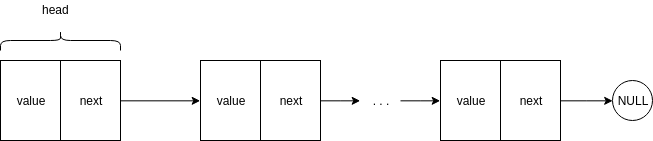
\includegraphics[width=1.00\textwidth]{Images/DataStructures/LinkedLists/SinglyLinkedList.png}
    \caption{Diagram of a singly linked list}
    \label{fig:singly_linked_list_diagram-01}
\end{figure}

\begin{lstlisting}
    struct Node{

        Node *next;
        int value;

        Node( int _value ){
            value = _value;
            next = NULL;
        }

    };

    typedef struct LinkedList{
        
        Node *tail;
        Node *head;
        int size;

        LinkedList(){
            tail = head = NULL;
            size = 0;
        }

        void insertAtTail(int value){
            Node *node = new Node( value );
            if( size > 0 ){
                tail -> next = node;
                tail = node;
            } else {
                tail = head = node;
            }
            size++;
        }

        void insertAtHead(int value){
            Node *node = new Node( value );
            if( size > 0 ){ 
                node -> next = head;
                head = node;
            } else {
                head = tail = node;
            }
            size++;
        }

        void Delete(int i){
            if( i < size && i >= 0 ){
                Node *aux = head;
                //If we want to delete the first element
                if( i == 0 )
                    head = head -> next;
                //If we want to delete the last element
                else if ( i == size ){

                    for( int j = 0; j <= size - 1; j++ )
                        aux = aux -> next;

                    aux -> next = NULL;
                    tail = aux;
        
                } else {
                    for( int j = 0; j < i - 1; j++)
                        aux = aux -> next;
                    aux -> next = aux -> next -> next;
                } 
                size--;
            }
        }

        void DeleteAtHead(){
            if( size == 1 )
                head = tail = head -> next; 
            else
                head = head -> next;
            size--;
        }

        int Search(int i){

            if( i < size ){
                Node *aux = head;
                for(int j = 0; j < i; j++)
                    aux = aux -> next;
                return aux -> value;
            }

            return INT_MIN;
        }

        bool isEmpty(){
            return ( size == 0 );
        }

        int getSize(){
            return size;
        }

        void print(){
            Node *aux = head;
            while( aux != NULL ){
                cout << aux -> value << "\t";
                aux = aux -> next;
            }
            cout << endl;
        }
    } LinkedList;
\end{lstlisting}

\subsection{Problems}
\subsubsection{Problem 01}
\textsf{Reverse a linked list}
\begin{lstlisting}
    #include <bits/stdc++.h>

    using namespace std;

    int main(){
        string s;
        int number_01 = 0, number_02 = 0;
        stack< int > Stack;
        cin >> s;

        for( auto c : s ){
            if( isdigit(c) ){
                Stack.push( c - '0' );
            } else {

                number_01 = Stack.top();
                Stack.pop();
                number_02 = Stack.top();
                Stack.pop();

                if ( c == '+')
                    Stack.push( number_02 + number_01 );
                else if ( c == '-' )
                    Stack.push( number_02 - number_01 );
                else if ( c == '*' )
                    Stack.push( number_02 * number_01 );
                else if ( c == '/' )
                    Stack.push( number_02 / number_01 );
            }
            
        }
        cout << Stack.top() << endl;
        return 0;
    }
\end{lstlisting}

\subsubsection{Problem 02}
\textsf{Detect a loop in a linked list}
\begin{lstlisting}
    #include <bits/stdc++.h>

    using namespace std;

    stack< int > StackSort(stack<int> &Stack){

        stack<int> AStack;
        
        while( !Stack.empty() ){
            int aux = Stack.top();
            Stack.pop();
            
            while( !AStack.empty() && AStack.top() > aux ){
    
                Stack.push( AStack.top() );
                AStack.pop();    

            }

            AStack.push( aux );
        }
        return AStack;
    }

    int main(){
        stack<int> Stack;
        int n, v;
        cin >> n;
        while(n--){
            cin >> v;
            Stack.push(v); 
        } 

        Stack = StackSort( Stack );

        while( !Stack.empty() ){
            cout << Stack.top() << endl;
            Stack.pop();
        }

        return 0;
    }
\end{lstlisting}

\subsubsection{Problem 03}
\textsf{Return N-th node from the end in a linked list}
Solve this problem is not difficult just you need to check which element between our two arrays is smaller than the other, and we will do this until one of our indexes is in the limit. Finally we need to check if one of our arrays was not checked completely. 
\begin{lstlisting}
    #include <bits/stdc++.h>

    using namespace std;

    int main(){

        int m, n;
        vector<int> M, N, ans;

        cin >> m >> n;
        M.resize(m, 0);
        N.resize(n, 0);

        for(int i = 0; i < m; i++)
            cin >> M[i];

        for(int i = 0; i < n; i++)
            cin >> N[i];

        int i = 0, j = 0;
        while( i < m && j < n ){
            if(M[i] < N[j]){
                ans.push_back( M[i++] );
            } else {
                ans.push_back( N[j++] );
            }
        }

        for ( ; i < m; i++)
            ans.push_back( M[i] );

        for( ; j < n; j++)
            ans.push_back( N[j] );

        for( auto e : ans )
            cout << e << " ";
        
        cout << endl;
        return 0;
    }
\end{lstlisting}

\subsubsection{Problem 04}
\textsf{Remove duplicates from a linked list}
To solve this problem we need something to help us, maybe we can use a bucket, but maybe we do not know the biggest number of an element inside the linked list, and also it makes to use a lot of memory so we can use hash to make this efficient in time and memory, in this case I gonna use an unordered set, it is a contianter that uses a hash to store efficientlly data, if you need more information about this you can show the \href{https://en.cppreference.com/w/cpp/container/unordered_set}{ \textbf{CPP reference} } and here is the solution for this problem.
\begin{lstlisting}
    #include <bits/stdc++.h>

    using namespace std;

    struct Node{
        Node *next;
        int value;
        Node(){
            next = NULL;
        }
    };

    Node *RemoveDuplicates( Node *head ){
        unordered_set<int> duplicates;
        Node *current = head;
        Node *previous = NULL;
        while(current -> next != NULL){

            if( duplicates.find( current -> value ) != duplicates.end() ){
                previous -> next = current -> next;
            } else {
                duplicates.insert( current -> value );
                previous = current;
            }
            current = current -> next;
        }

        return head;
    }

    void printList( Node *head ){
        Node *aux = head;
        cout << endl;
        while( aux -> next != NULL ){
            cout << aux -> value << " ";
            aux = aux -> next;
        }
        cout << endl;
    }

    int main(){
        int n, v;
        Node *head = new Node();
        Node *aux = head;

        cin >> n; 
        while(n--){
            cin >> aux -> value;
            aux -> next = new Node();
            aux = aux -> next;
        }

        printList( head );

        aux = RemoveDuplicates( head );

        printList( aux );
        
        return 0;
    }
\end{lstlisting}
